\subsection{Centralized Algorithms}
\label{sec:centralizedsolution}
Two centralized algorithms are proposed to solve our clustering problem. These two algorithms use the similar idea of the greedy algorithm for the set cover problem but adopt different approaches to handle the extra constraints of clustering. In both of the algorithms, a set of candidate single-hop clusters is first established given the network  \(G =(V,E)\). Then the most cost-effective cluster is selected from this set, one at a time, until all the sensor nodes in \(V\) have been covered.  

In the first algorithm, to find a candidate cluster set \(U\), we first calculate the optimal cluster size \(n_{opt}\) according to Eq. \ref{eq:MagicNumberOverlapping2}. Then based on \(n_{opt}\), one-hop neighbors of each node in \(V\) are partitioned. For each node \(s_i \in V\), assume the one-hop neighbor set is \(Ne_{s_i}\), if \( \left|Ne_{s_i}\right| \geq n_{opt}-1\), then each cluster in the cluster set contains a common element \(s_i\) and the remaining elements are the combinations of nodes in \(Ne_{s_i}\) with the length of \(n_{opt}-1\). When \(\left|Ne_{s_i}\right| < n_{opt} -1\), \(C_i =\{s_i\} \bigcup Ne_{s_i}\). Note that we assume the network is dense enough such that each sensor node has at least \(p\) one-hop neighbors. The obtained cluster sets for all the nodes in \(V\) are combined together to obtain the candidate cluster set \(U\).

The algorithm then selects the most cost-effective cluster \(S_i \in U\), one at a time, until all the sensor nodes in \(V\) have been covered. The cost effectiveness, denoted as \(\lambda\), is defined as \(\lambda = \frac{1}{\left|S_i\cup C_a\right| - \left|C_a\right|}\), where \(C_a\) represents the set of nodes covered so far. When selecting the most cost-effective cluster, we choose from the clusters in \(U\) which overlap with \(C_a\). This strategy can ensure that all the selected sensor nodes will be connected through the overlapping nodes.  If more than one candidate clusters which overlap with \(C_a\) have the same \(\lambda\), the one which maximizes the total degrees of the remaining un-covered nodes (i.e. \(U- S_i\bigcup C_a\)) will be chosen. It can be seen that this algorithm divides the sensor nodes in \(V\) into as many single-hop clusters of size \(n_{opt}\) as possible while keeps the number of overlapping nodes into minimums (from \(\lambda = \frac{1}{\left|S_i\cup C_a\right| - \left|C_a\right|}\), penalty is given to cluster having large number of overlapping nodes with \(C_a\)). Both of these two points are of importance to minimize the overall energy cost. The algorithm is shown as Algorithm \ref{algo:greedy1}.

The second algorithm uses different strategy to handle overlapping.  First, the optimal cluster size \(n_{opt}\) is calculated based on Eq. \ref{eq:MagicNumberOverlapping} without considering overlapping constraint. When selecting the most cost effective cluster, it is chosen from all the candidate clusters in \(U\). Since the overlapping constraint is not considered when selecting cluster, after all the sensor nodes in \(V\) have been covered, the algorithm will test if all the clusters are connected through the overlapping nodes and add extra clusters to connect them if necessary. The basic idea is to identify all the isolated cluster groups and then find clusters to connect them. The detailed description is omitted for brevity. This algorithm is shown as Algorithm \ref{algo:greedy2}. 

\begin{comment}
To achieve this, all the isolated cluster groups (ICGs) from the obtained clusters are identified . Clusters within an ICG are connected through overlapping nodes but do not overlap with other ICGs. Each ICG is then represented as a vertex in a graph \(G_{ICG}\). There is an edge between two vertices in \(G_{ICG}\) if there exist two nodes, each within a ICG corresponding to one of the two vertices, are within the communication range of each other. Then the minimum spanning tree (MST) is found that can connect all the vertices in \(G_{ICG}\). For each edge in the MST, an extra cluster is established in which the two sensor nodes associated with the edge are included. If \(p \geq 2\), then additional nodes should also be added to satisfy the constraint 3 of the optimal clustering problem. This algorithm is shown as Algorithm \ref{algo:greedy2}.
\end{comment}

\begin{algorithm}
\begin{algorithmic}[1]
\REQUIRE \(G=(V, E)\) and parameters listed in Table. \ref{tab:Table2}
\STATE find \(n_{opt}\) which minimizes Eq. \ref{eq:MagicNumberOverlapping}
	\STATE \(U\gets \emptyset\) \(C_a\gets \emptyset\)
	\FORALL {\(n_i\in V\)}
		\STATE \(S_i\gets \emptyset\)
		\FORALL {one hop neighbor \(n_j\) of \(n_i\)}
			\STATE \(S_i = S_i \bigcup \{n_j\}\)
		\ENDFOR
		\STATE construct a cluster set \(C_i\) whose elements are the combinations taken of the nodes in \(S_i\) of length \(n_{opt} - 1\).
		\STATE \(U=U\bigcup C_i\)
	\ENDFOR
	 	\REPEAT
	 \STATE \(C_{cand} =\) all the clusters in \(U\) which overlap with \(C_a\)
		\STATE find a cluster \(S_i\) in \(C_{cand}\) with the smallest \(\frac{1}{\left|S_i\cup C_a\right| - \left|C_a\right|}\)
		\STATE \(C_a=C_a\bigcup S_i\)	
		\UNTIL {\(C_a\) covers \(V\)}
	\ENSURE \(C_a\)
\end{algorithmic}
\caption{First centralized algorithm for clustering}
\label{algo:greedy1}
\end{algorithm}

\begin{algorithm}
\begin{algorithmic}[1]
\REQUIRE \(G=(V, E)\) and parameters listed in Table. \ref{tab:Table2}
\STATE find \(n_{opt}\) which minimizes Eq. \ref{eq:nooverlap}
  \STATE The same with the 2 to 16 lines of Algorithm \ref{algo:greedy1}
  	\REPEAT
		\STATE find a cluster \(S_i\) in \(U\) with the smallest \(\frac{1}{\left|S_i\cup C_a\right| - \left|C_a\right|}\)
		\STATE \(C_a=C_a\bigcup S_i\)
	\UNTIL {\(C_a\) covers \(V\)}
	\STATE Identify Isolated cluster groups (ICGs) in \(C_a\)
	\STATE Construct a graph \(G_{ICG}=(V_{ICG}, E_{ICG})\):
 \STATE Run MST algorithm on \(G_{ICG}\) and get \(T\)
	\FORALL {edges in \(T\)}
		\STATE Create an extra cluster \(C_e\) and add it to \(C_a\)
	\ENDFOR
	\ENSURE \(C_a\)
\end{algorithmic}
\caption{Second centralized algorithm for clustering}
\label{algo:greedy2}
\end{algorithm}

\begin{comment}
We will use a simple example to demonstrate the two algorithms above. Figure \ref{fig:AlgorithmExampleNew}(a) plots a graph consisting of a total of 12 nodes. Assume we use the parameters associated with energy listed in Table 1 and the optimal \(n_{opt}\)=4. For simplicity, we also assume that the \(cond(S_i)<\gamma\) if \(\left|S_i\right| \geq p = 3\). Using the generated candidate cluster sets, 4 clusters are obtained using the first algorithm and illustrated in Figure \ref{fig:AlgorithmExampleNew}(b). Note that all these 4 clusters are connected through the overlapping nodes. Using the second algorithm, a total of 3 clusters are generated after all the 12 nodes have been covered (see Figure \ref{fig:AlgorithmExampleNew}(c)). However, these clusters do not overlap. Therefore, two extra clusters are generated to connect these isolated clusters. Note that since the minimum number of vibration patterns is 3, each extra cluster contains three nodes. The final clustering result of the second algorithm is shown in Figure \ref{fig:AlgorithmExampleNew}(d). The total amount of energy using the generated clusters from the first algorithm is about \(0.88\) times of that of the second algorithm. 

\begin{figure}
	\centering
		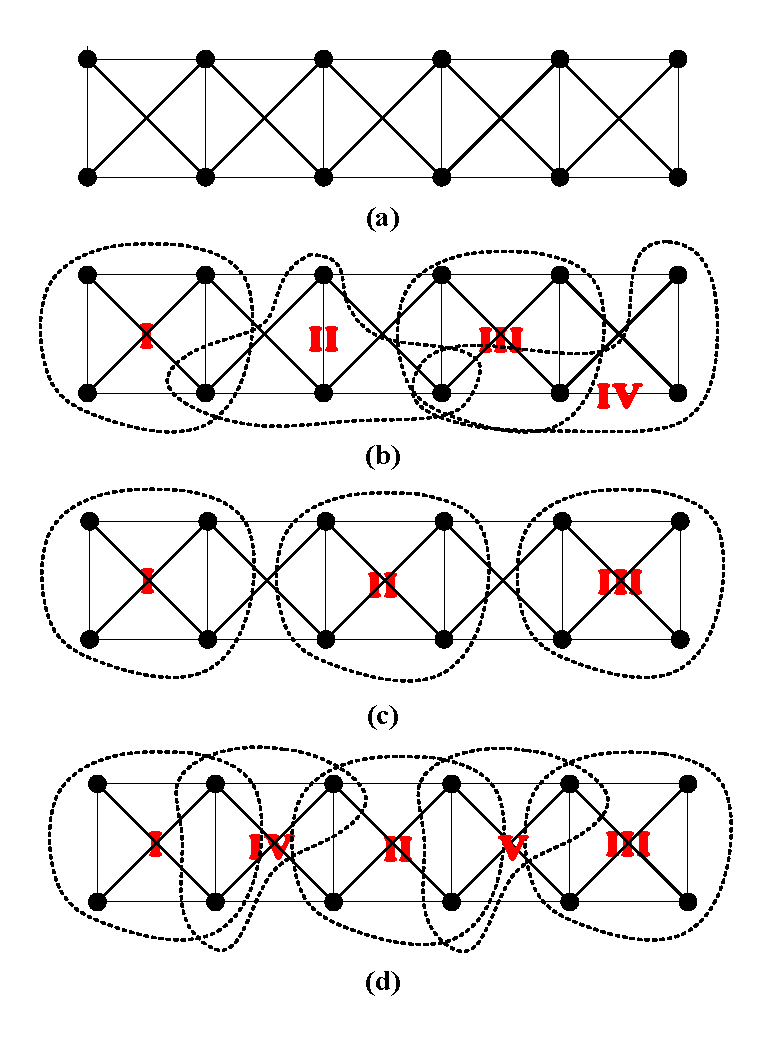
\includegraphics[width=.3\textwidth,height=.35\textwidth]{AlgorithmExampleNew.eps}
	\caption{Example of using the Proposed Algorithms (a) Graph G(V,E), (b) The 4 Clusters Generated from the \(1^{st}\) Algorithm (c) Isolated Cluster Groups from the \(2^{nd}\) Algorithm (e) Final 5 Clusters from the \(2^{nd}\) Algorithm}
	\label{fig:AlgorithmExampleNew}
\end{figure}
\end{comment}

